\documentclass{article}
\usepackage[utf8]{inputenc}
\usepackage[margin=2cm,a3paper,landscape]{geometry}
\usepackage{multicol}
\usepackage[svgnames]{xcolor}
\usepackage{float}
\usepackage{graphicx}
\usepackage{booktabs}

\usepackage{amsmath}
\makeatletter
\g@addto@macro\normalsize{%
  \setlength\abovedisplayskip{.4cm}
  \setlength\belowdisplayskip{.4cm}
  \setlength\abovedisplayshortskip{.4cm}
  \setlength\belowdisplayshortskip{.4cm}
}
\makeatother

\definecolor{headercolor}{RGB}{0,80,158}

\usepackage{titlesec}

\titleformat{\section}
{\color{headercolor}\normalfont\Large\bfseries}
{\color{headercolor}\thesection}{1em}{}

% Paragraphs skips one line and don't indent
\setlength{\parindent}{0em}
\setlength{\parskip}{1em}

% Don't show page numbers
\pagenumbering{gobble}

\usepackage[backend=biber,style=numeric,sorting=ynt,block=ragged]{biblatex}
\addbibresource{references.bib}

\begin{document}

\begin{minipage}[b]{0.80\linewidth}

{\color{headercolor}\Huge Automotive Embedded System Implementation Using System-on-Module}\\[.5cm] % Title
\LARGE \textbf{By Trym Sneltvedt}\\ % Author(s)
\LARGE Department of Informatics and Electronics, Norwegian University of Technology and Science\\ % University/organization
\LARGE Supervised by Bjørn B. Larsen

\end{minipage}
%
\begin{minipage}[t]{0.10\linewidth}

\includegraphics[width=2.5cm]{media/ntnu_alt_versjon_uten_slagord.png}
\end{minipage}
%
\begin{minipage}[t]{0.10\linewidth}

\includegraphics[width=2.5cm]{media/revolve_standing.png}
\end{minipage}

\vspace{1cm}

% Poster body
\begin{multicols}{3}


%\section*{Abstract}
\section*{Introduction}

Revolve NTNU is a student organization participating in the international Formula Student competitions, designing and constructing and competing with electric vehicles.

% The combination of short development time and automotive embedded electronics introduces interesting problems. This report will focus on a specific embedded system, the VCU, and the issues encountered when developing it. As the electric vehicle is almost exclusively made from custom parts, the different systems on the car depends heavily on each other. This means that changes done to the VCU will invariably affect the rest of the vehicle and vice-versa. 

\begin{figure}[H]
    \centering
    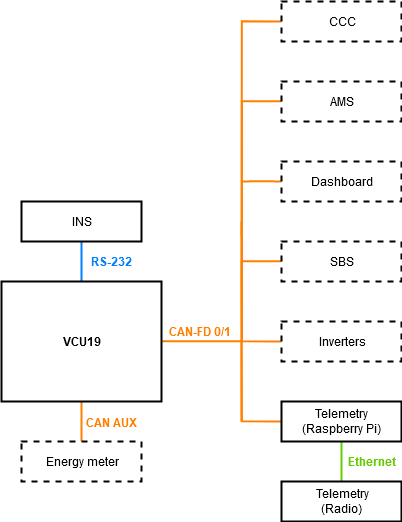
\includegraphics[width=.45\linewidth]{media/vcu19_system_2.png}
    \caption{Communication architecture 2019}
    \label{fig:comarch_old}
\end{figure}

This project details the design of a Vehicle Control Unit (\emph{VCU}) for the 2020 season of Formula Student. The new design is based on the design from the 2019 season, where the VCU switched from a Microchip ATSAM based design to the Xilinx Zynq-7000 System-on-Chip platform. The previous communication architecture is detailed in figure \ref{fig:comarch_old}.


\section*{Method}

Special attention has been brought to the CAN-FD (Controller Area Network Flexible Data-rate) buses used for communication. As more systems are added to the vehicle every year, the load of the buses is of great importance. To improve and future-proof the partitioning of the buses, a simple utilization based schedulability test is used to determine whether the bus can guarantee that all messages are sent, see (\ref{eq:utilization_criteria}).

\begin{equation}
    U=\sum_{i=1}^N\frac{C_i}{T_i}\leq N\left(2^\frac{1}{N}-1\right)
    \label{eq:utilization_criteria}
\end{equation}

This equation gives a maximum utilizitation of $69.4\%$ for a significant amount of frames on the bus. A Python script is used to calculate the worst case load for each bus, allowing for improved partitioning. %we get an overview of the bus load on both buses.

% As arbitration of messages (or \emph{frames}) on a CAN-FD bus are handled by recessive bits in the message identifier, frames are sent consecutively one after another without break. This is the reason we can use the schedulability test from real-time theory. 


\section*{Results}

The results of the simulated worst case bus load is shown in figure \ref{fig:utilization}.

\begin{figure}[H]
    \centering
    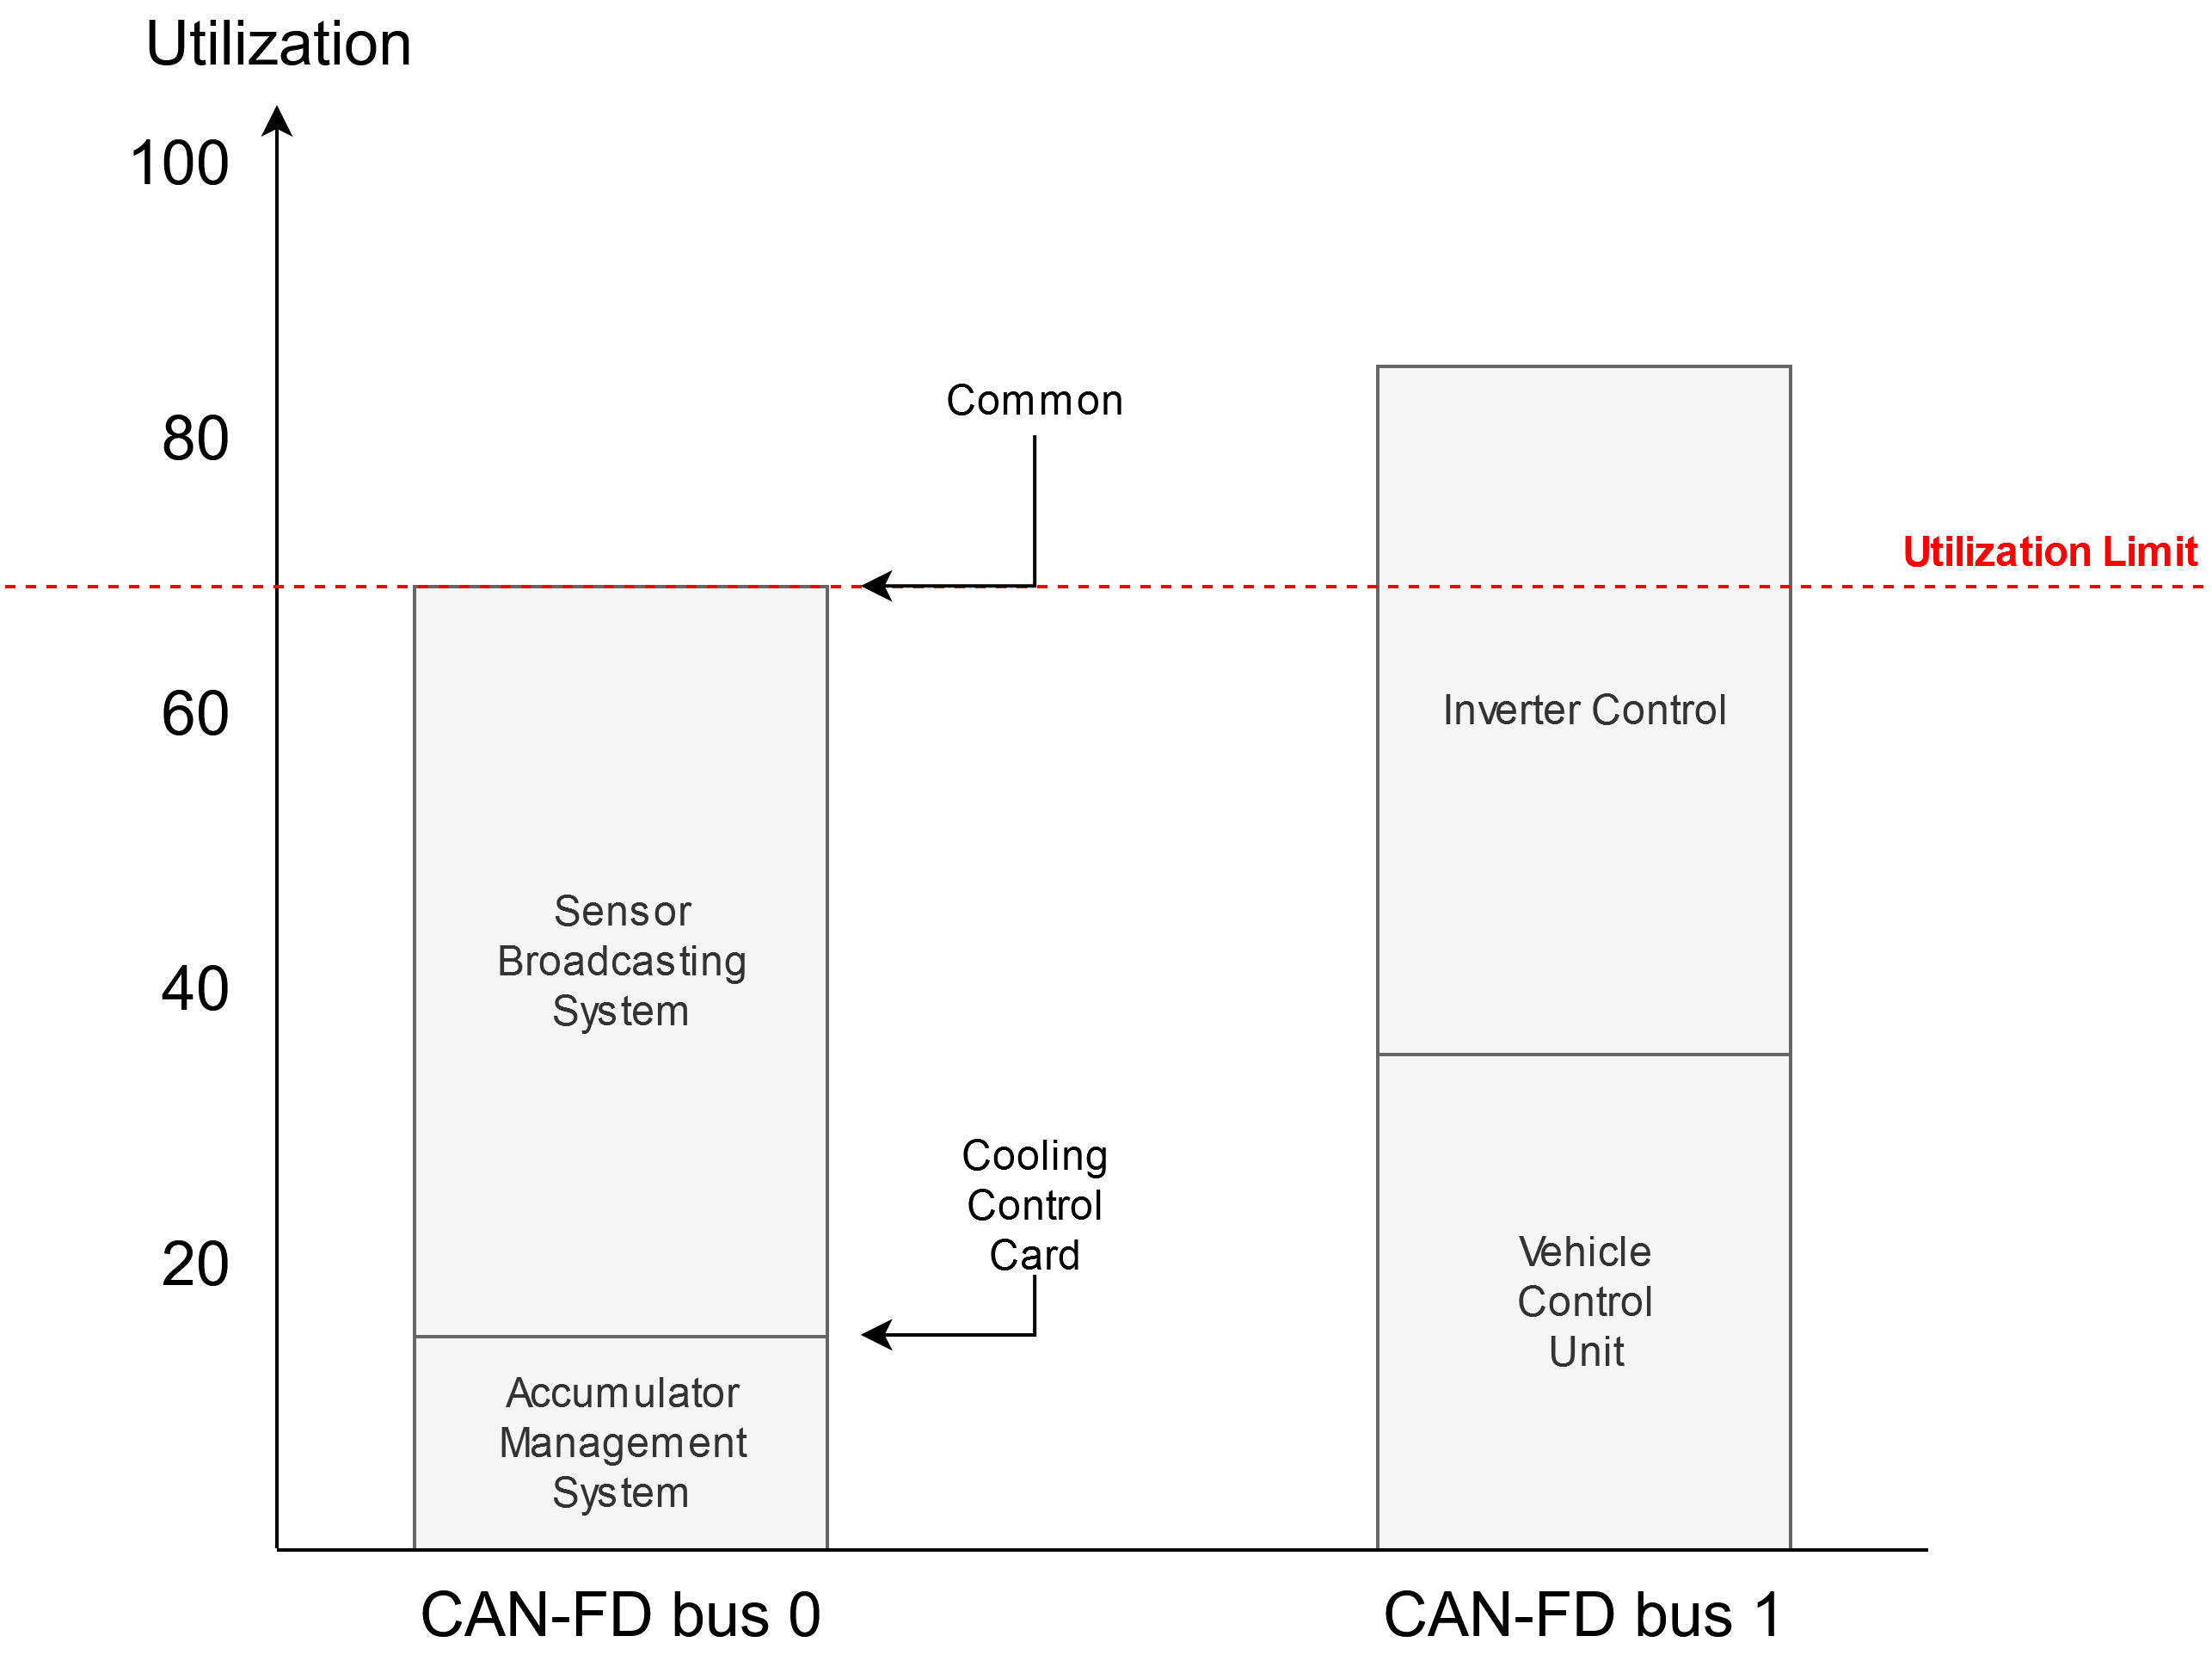
\includegraphics[width=.75\linewidth]{media/utilization.png}
    \caption{Utilization on both CAN-FD buses}
    \label{fig:utilization}
\end{figure}

\begin{figure}[H]
    \centering
    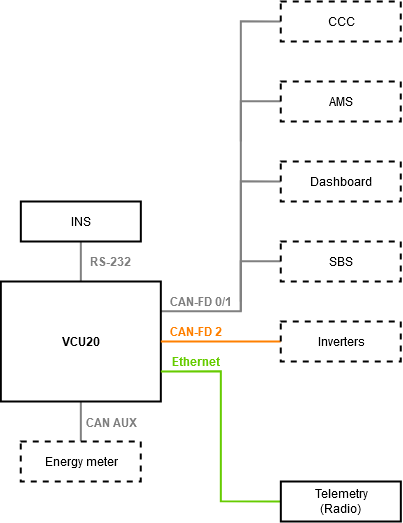
\includegraphics[width=.45\linewidth]{media/vcu20_system_2.png}
    \caption{New communication architecture}
    \label{fig:comarch_new}
\end{figure}

The results indicated that there is need for more CAN-FD buses. Along with this, the SoM has support for Ethernet, which allows the removal of the former Raspberry Pi based telemetry solution, saving weight and bus load. These changes leads to the new communication architecture shown in figure \ref{fig:comarch_new}.

The finished PCB has been soldered and functionally tested. Aside from a few "bugs" the system functions correctly and provides a solid platform for a VCU in the 2020 season. As the project is far from finished, all aspects of the system has not been tested and the details are subject to change.


\section*{Conclusion}

\begin{figure}[H]
    \centering
    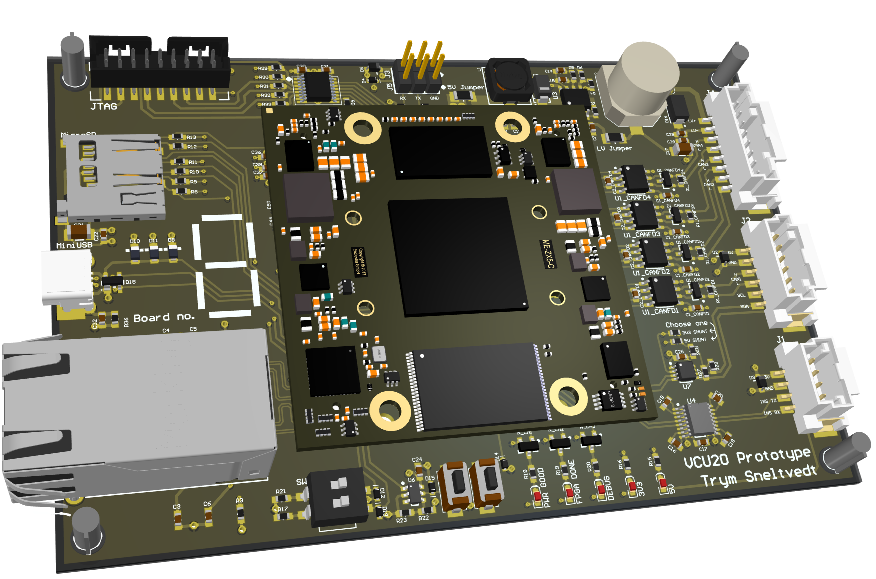
\includegraphics[width=.7\linewidth]{media/vcu20_proto_render.png}
    \caption{3D render of finished VCU PCB.}
    \label{fig:render}
\end{figure}

A VCU built around an Enclustra Mercury ZX5 SoM was successfully designed and tested, this results in simpler hardware design, increasing maintainability and robustness. And by using the an Ethernet interface along with changing the partitioning of the CAN-FD buses, the load is reduced to a safe level allowing for further additions to the bus. The finished VCU can be seen in figure \ref{fig:render}. \cite{this}

%This project details the design of a hardware platform thought to serve as a Vehicle Control Unit (VCU) for an electric Formula Student Race car. Special attention was given to reducing the development and production costs of using a Zynq-7000 System-on-Chip by transitioning to a System-on-Module. Other changes in the design was motivated by closer analysis of the communication architecture in the vehicle 


% References
\addcontentsline{toc}{section}{References}
\printbibliography

\end{multicols}

\end{document}
